\documentclass{beamer}
\DeclareFontShape{OT1}{cmss}{b}{n}{<->ssub * cmss/bx/n}{} 
\usetheme{default}
\usepackage{amsmath}
\usepackage{amsfonts}
\usepackage{mathbbol}
\usepackage{xcolor} % before tikz or tkz-euclide if necessary
\usepackage{tkz-euclide} % no need to load TikZ
\usepackage{multirow}
\usepackage{lmodern}
\usepackage{bm}

\usepackage[
backend=biber,
style=authoryear-icomp,
sortlocale=de_DE,
natbib=true,
url=false, 
doi=true,
eprint=false
]{biblatex}
\addbibresource{../../Bibliography/main_ML.bib}



\titlegraphic{
\includegraphics[width=2cm]{../../Figures/UAMS_RGB.png}
}


\title{Statistical Machine Learning\\ Finding Minima Algorithms}
\author{Horacio G\'omez-Acevedo\\ Department of Biomedical Informatics\\
	University of Arkansas for Medical Sciences}
\begin{document}
	\begin{frame}[plain]
		\maketitle
	\end{frame}
	
	\begin{frame}{Case $n=1$}
		Let's suppose we have a real valued function which is smooth $f\colon \mathbb{R}\to \mathbb{R}$. Then, we can approximate the function in a vicinity of $x=c$ by the so-called Taylor expansion
		\begin{equation*}
			f(x)= f(c)+ \frac{df}{dx}(c) (x-c)+  \frac{1}{2!} \frac{d^2f}{dx^2}(c) (x-c)^2 +  \frac{1}{3!} \frac{d^3f}{dx^3}(c) (x-c)^3+ \cdots
		\end{equation*}
		Notice that when $x$ is very close to $c$, then $(x-c)^p$ for $p\ge 3$ starts getting exceedingly small. Then, we write 
			\begin{equation*}
			f(x) \approx f(c)+ \frac{df}{dx}(c) (x-c)+  \frac{1}{2!} \frac{d^2f}{dx^2}(c) (x-c)^2 
		\end{equation*}
		
		If at the point $x=c$ the function reaches a (local) minimum, then $f'(c)=0$.
		
		Recall that in the threshold logic,  once we receive the input, a decision must be made to \textit{fire} or \textit{suppress} the output. 
		
		
		\textbf{Activation functions} generalize the concept of activation given a specific  input.
		
		
	\end{frame}
	\begin{frame}{Case $n\ge 2$}
	Let's suppose we have a real valued function which is smooth $f\colon \mathbb{R}^n\to \mathbb{R}$. Then, we can approximate the function in a vicinity of $x=c$ by the so-called Taylor expansion
	\begin{equation*}
		\begin{split}
	f(\textbf{x}) &= f(\textbf{c})+ \sum_i \frac{\partial f}{\partial x_i}(c) (x_i-c_i)+  \frac{1}{2!} \sum_{i,j}\frac{\partial^2f}{\partial x_i \partial x_j}(c) (x_i-c_i)(x_j-c_j) +   \cdots\\
	&\approx f(\textbf{c})+ (\textbf{x}-\textbf{c})^T \nabla f(\textbf{c})+ \frac{1}{2} (\textbf{x}-\textbf{c})^T H_f(\textbf{c}) (\textbf{x}-\textbf{c})\\
		\end{split}
	\end{equation*}


	Where $H_f(\textbf{c})$ is the \textbf{Hessian matrix} defined as 
	\begin{equation*}
		H_f(\textbf{c})= \begin{pmatrix}
			\frac{\partial^2 f}{\partial x_1 \partial x_1} (\textbf{c}) & 	\frac{\partial^2 f}{\partial x_1 \partial x_2} (\textbf{c}) & \cdots & 	\frac{\partial^2 f}{\partial x_1 \partial x_n} (\textbf{c}) \\
				\frac{\partial^2 f}{\partial x_2 \partial x_1} (\textbf{c})  & 	\frac{\partial^2 f}{\partial x_2 \partial x_2} (\textbf{c}) & \cdots & 	\frac{\partial^2 f}{\partial x_2\partial x_n} (\textbf{c})\\
				\vdots & \vdots & \ddots & \vdots\\
					\frac{\partial^2 f}{\partial x_n \partial x_1} (\textbf{c}) & 	\frac{\partial^2 f}{\partial x_n  \partial x_2} (\textbf{c}) & \cdots &	\frac{\partial^2 f}{\partial x_n \partial x_n} (\textbf{c})      
		\end{pmatrix}
	\end{equation*}
\end{frame}

\begin{frame}{Minimum Condition}
	For the case $n=1$, the point $x=c$ if $f'(c)=0$ and $f''(c)<0$, then the function $f$ has a \textbf{local minimum} at $c$. 
	
	For the case when $n\ge 2$, if $\nabla f(\textbf{c})=0$ and that $H_f$ satisfies for points close to $\textbf{c}$
	\begin{equation*}
		v^T H_f  v >0 \; \forall v \in \mathbb{R}^n -\{0\}
	\end{equation*}
	Then, $\textbf{c}$ is a \textbf{local minimum} of $f$.
\end{frame}
	
	\begin{frame}{Linear Functions}
		
		These functions are used to model the firing rate of a neuron.
		
		\begin{equation*}
			f(x)= kx \quad k \text{ is a positive constant}
		\end{equation*}
		
		Pros: It is continuous and differentiable.	
		
		\begin{figure}[h]
			\centering
			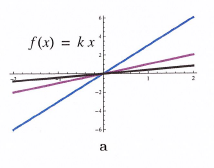
\includegraphics[scale=0.8]{../../Figures/fig_activation_21.png}
		\end{figure}
		
		
	\end{frame}

\begin{frame}{References}
	Materials and some of the pictures are from \citep{calin}.
	\printbibliography 	
	
	I have used some of the graphs by hacking TiKz code from StakExchange, Inkscape for more aesthetic plots and other old tricks of \TeX
	
\end{frame}


\end{document}
